\documentclass[10pt]{beamer}

\usetheme[progressbar=frametitle]{metropolis}
\usepackage{appendixnumberbeamer}

\usepackage{booktabs}
\usepackage[scale=2]{ccicons}

\usepackage{pgfplots}
\usepgfplotslibrary{dateplot}
\usepackage{comment}
\usepackage{xspace}
\usepackage{graphicx} 
\usepackage{subcaption}
\usepackage{subcaption}

\newcommand{\themename}{\textbf{\textsc{metropolis}}\xspace}

\title{Particle transport due to electrostatic waves}
\date{\today}
%\date{}
\author{André Farinha Bósio}
\institute{Instituto de Física - Universidade de São Paulo \\ Marseille, Nov. 7, 2023}
\titlegraphic{
\hfill
\includegraphics[height=1cm]{if.png}
\hfill
\includegraphics[height=1cm]{Identidade_Visual_CAPES.png}
\hfill
\includegraphics[height=1cm]{aix.jpg}
\hfill
\includegraphics[height=1cm]{piim.png}
\hfill
\includegraphics[height=1cm]{mesocentre.png}
\hfill
\includegraphics[height=1cm]{Logo-CNRS.png}

}



%\usepackage[brazilian]{babel}
\usepackage[english]{babel}

\begin{document}

\maketitle

\begin{frame}{Topics}
  \setbeamertemplate{section in toc}[sections numbered]
  \tableofcontents%[hideallsubsections]
\end{frame}



\section{Introduction}

\begin{frame}{Introduction}


\begin{itemize}

\item Plasmas
\item Tokamaks
\item Edge transport

\end{itemize}

\end{frame}

\begin{frame}{Plasma confinement}

\begin{figure}[h]
\centering
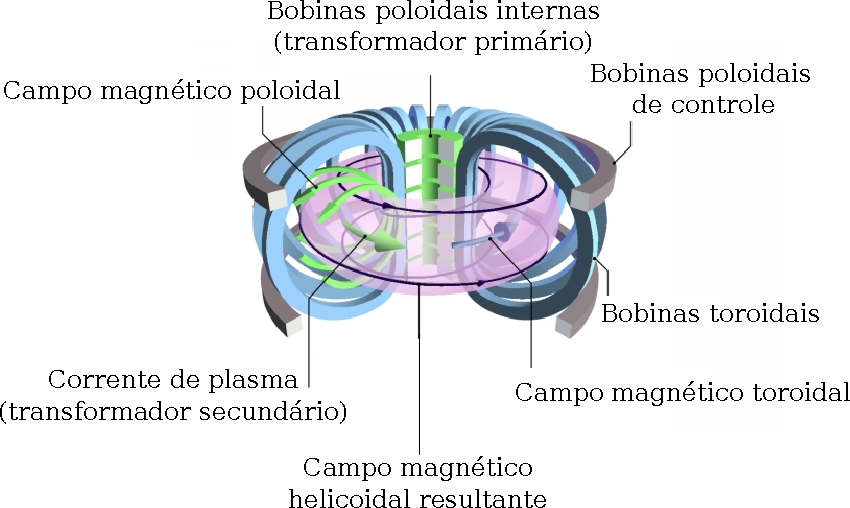
\includegraphics[width = 0.8\textwidth]{imgs/tokamak.pdf}
\caption{The magnetic fields due to the coils}
\label{tokamak}
\end{figure}

\end{frame}

\section{$E \times B$ drift}

\begin{frame}{$\vec{B} = B\hat{z}$ and $\vec{E} = 0$}
 
\begin{equation}
\vec{F} = m \frac{d \vec{v}}{dt} = q(\vec{v}\times \vec{B})
\label{Lorentz}
\end{equation}

and

\begin{equation}
x-x_0 = r_L \sin(\omega_c t) \hspace{1 cm} y-y_0 = r_L \cos(\omega_c t)
\end{equation}

$x_0$ e $y_0$ are the guiding centers of the motion.

$\omega_c$ and $r_L$ are the gyrofrequency and the Larmor radius.

\begin{equation}
\omega_c = \frac{|q|B}{m}      \hspace{1cm}  r_L = \frac{m v_{\perp}}{|q|B}
\end{equation}

\end{frame}


\begin{frame}{$\vec{B} = B\hat{z}$ and uniform $\vec{E}$} 

Along $\hat{z}$:
\begin{equation}
    \dot{v}_z = \frac{q}{m}E_z \rightarrow v_z = \frac{qE_z}{m}t + v_{z0}
\end{equation}

In $x-y$ plane:
\begin{equation}
m\dot{v}_x = \frac{q}{m}E_x + \omega_c v_y  qBv_y \hspace{1 cm} m\dot{v}_y = qBv_x 
\end{equation}

\begin{equation}
v_x = v_{\perp} e^{i\omega_c t} \hspace{1 cm} v_y = iv_{\perp} e^{i\omega_c t} - \frac{E_x}{B}
\end{equation}
\begin{equation}
    v_\perp = \sqrt[2]{v_x^2 + v_y^2}
\end{equation}

with drift velocity

\begin{equation}
\vec{v}_E = \frac{\vec{E}\times \vec{B}}{B^2}
\end{equation}

\end{frame}

\begin{frame}{Illustration of the $E \times B$ drift}

\begin{figure}[h]
\centering
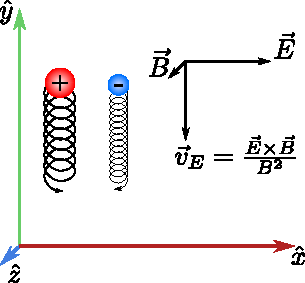
\includegraphics[width = 0.5\textwidth]{imgs/deriva.pdf}
\caption{Electric drift for two different kinds of particles}
\label{deriva}
\end{figure}

\end{frame}

\begin{frame}{Hamiltonian model model for the guiding centers}

\begin{equation}
\vec{B} = B_0 \vec{z} \hspace{1cm} \vec{E} = - \nabla \phi(x,y,t)
\end{equation}

\begin{equation}
\vec{v}_E = \frac{\vec{E} \times \vec{B}}{B^2}    
\label{eqderiva}
\end{equation}

\begin{equation}
v_x = \frac{dx}{dt} = -\frac{1}{B_0}\frac{\partial}{\partial y} \phi(x,y,t) \hspace{1cm} v_y = \frac{dy}{dt} = \frac{1}{B_0}\frac{\partial}{\partial x} \phi(x,y,t)
\end{equation}

\begin{equation}
\frac{dx}{dt} = -\frac{\partial}{\partial y} H(x,y,t) \hspace{1cm}  \frac{dy}{dt} = \frac{\partial}{\partial x} H(x,y,t)
\label{eqvs}
\end{equation}

\begin{equation}
H(x,y,z) = \frac{\phi(x,y,z)}{B_0}
\end{equation}

$x$ and $y$ are canonical conjugates

\end{frame}

\begin{frame}{Potential and reference frame}


\begin{equation}
\phi(x,y,t) = \phi_0(x) + \sum_i A_i \sin(k_{xi}x + \theta_{xi})\sin(k_{yi}y - \omega_i t + \theta_{yi})
\label{Potencial}
\end{equation}

For a single wave:

\begin{equation}
H(x,y,t) = \phi_0(x) + A_1 \sin(k_{x1}x)\sin(k_{y1}y - \omega_1 t)
\end{equation}

Change the reference frame through the canonical transformation:

\begin{equation}
F_2(x',y) = x'(y-v_1 t) \hspace{0.5cm} v_1 = \frac{\omega_1}{k_{y1}}
\end{equation}




\end{frame}


\begin{frame}{Equations of motion for a single wave}

\begin{equation}
H(x,y) = \phi_0(x) - v_1x + A_1 \sin(k_{x1}x)\sin(k_{y1}y)
\end{equation}

\begin{equation}
\frac{dx}{dt} = -k_{yi}A_i \sin(k_{xi}x)\cos(k_{yi}y)
\end{equation}

\begin{equation}
\frac{dy}{dt} =  \left[\frac{d\phi_0}{dx}  -  v_1\right] + k_{xi}A_i \cos(k_{xi}x)\sin(k_{yi}y)
\label{eqdy}
\end{equation}

\end{frame}


\begin{frame}{Control parameter $U(x)$}
    We can also define a control profile $U(x)$:

\begin{equation}
U(x) =  \frac{1}{A_1 k_{x1}} \left[ \frac{d\phi_0}{dx}  -  B_0v_1\right] = \frac{B_0}{A_1k_{kx1}} \left[ -\frac{E(x)}{B_0} - v_1  \right]
\label{eqU}
\end{equation}

\begin{equation}
    U(x) =  \frac{B_0}{A_1k_{x1}} \left[ v_E(x) - v_1  \right]
    \label{eqU2}
\end{equation}

When $U = 0$, we have a resonance, where the phase velocity of the wave is the same as the electric drift.

From now on $U(x) = U = cte$
\end{frame}





\begin{frame}{About some parameters $k_x$, $k_y$}

Restrictions on $k_x$ and $k_y$ to satisfy space periodicity:

\begin{equation}
k_{y} = \frac{2 \pi n}{L_y}  \hspace{1cm} k_{x} = \frac{2\pi m }{L_x} \hspace{1cm} n,m \in \mathbf{Z}
\end{equation}

with $L_x$ and $L_y$, being the $x$ and $y$ period. 

$L_{x,y} = 2\pi$ so that $k_{x,y}$ are integers

In the resonance, $U=0$, the trajectories structure themselves with a lattice of elliptic and hyperbolic points

\begin{equation}
P_H = \left(\frac{(2m+1)\pi}{2k_x};\frac{(2n+1)\pi}{2k_y}\right) \hspace{1cm} P_E = \left(\frac{m\pi}{k_x};\frac{n\pi}{k_y}\right)
\end{equation}



\end{frame}


\begin{frame}{Trajectories}
As $|U|$ increases, the structure of the cells changes

\begin{figure}[h]
\begin{subfigure}[b]{0.3\textwidth}
    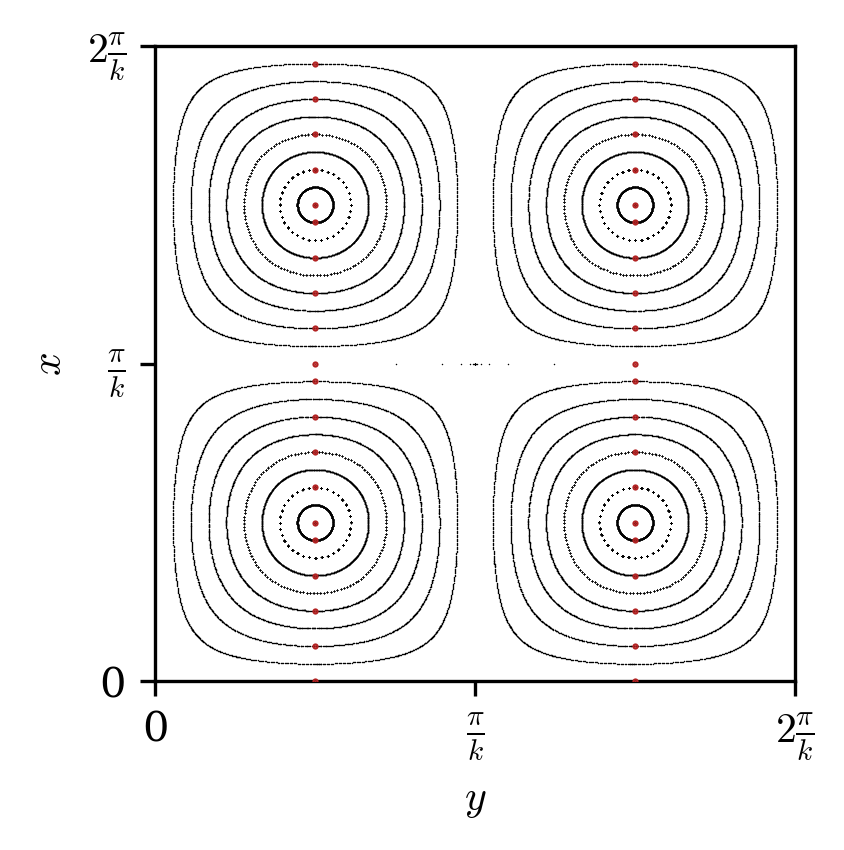
\includegraphics[width=\textwidth]{graf_1onda/map2_data-map2_U_p0.0000.png}
    \caption{$U = 0.0$}
\end{subfigure}
\begin{subfigure}[b]{0.3\textwidth}
    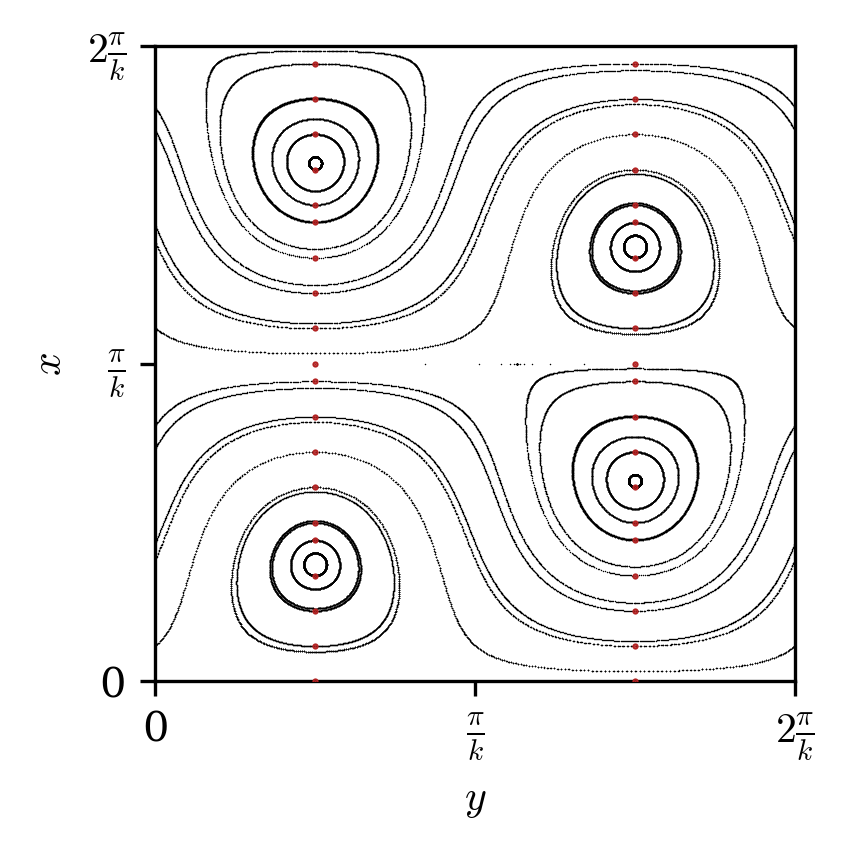
\includegraphics[width=\textwidth]{graf_1onda/map2_data-map2_U_p0.4000.png}
    \caption{$U = 0.4$}
\end{subfigure}
\begin{subfigure}[b]{0.3\textwidth}
    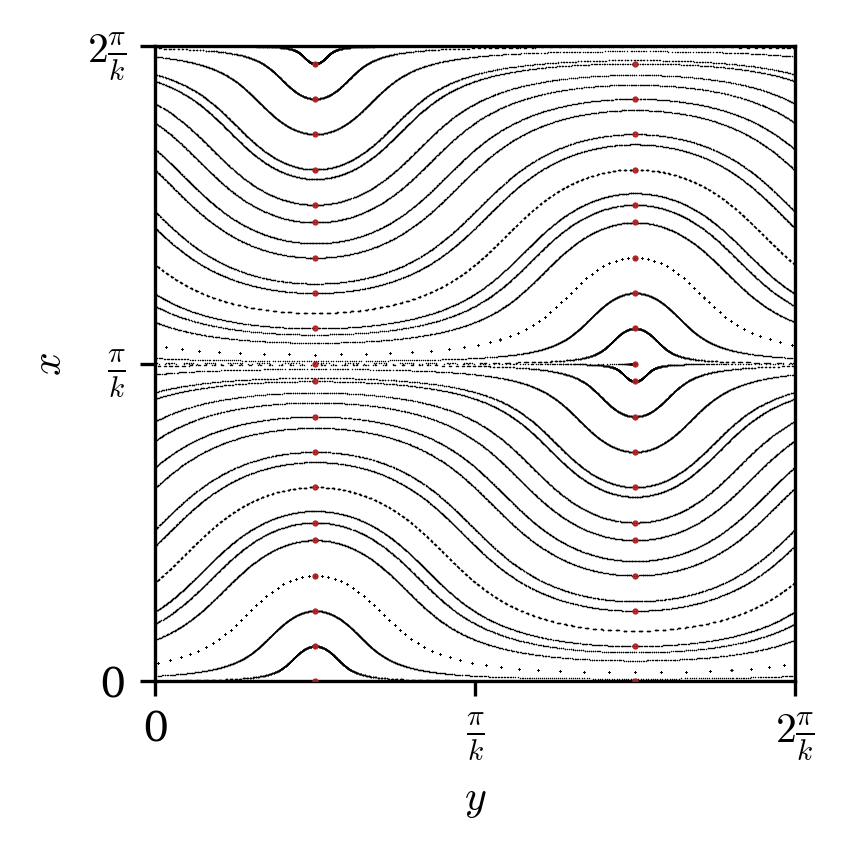
\includegraphics[width=\textwidth]{graf_1onda/map2_data-map2_U_p1.0000.png}
    \caption{$U = 1.0$}
\end{subfigure}

\caption{Guiding centers trajectories for a single wave}
\end{figure}

\end{frame}



\section{Two wave hamiltonian}

\begin{frame}{Hamiltonian}

\begin{equation}
H(x,y,t) = \phi_o + A_1 \sin(k_{x1}x)\sin(k_{y1}y - \omega_1t) + A_2 \sin(k_{x2}x + \theta_x)\sin(k_{y2}y - \omega_2t)
\label{2waveh}
\end{equation}

With the new reference frame 

\begin{equation}
H(x,y,t) = \phi_o - v_1x + A_1 \sin(k_{x1}x)\sin(k_{y1}y) + A_2 \sin(k_{x2}x + \theta_x)\sin(k_{y2}(y - vt))
\label{2waveh}
\end{equation}

\begin{equation}
    v = \frac{\omega_2}{k_{y2}} - \frac{\omega_1}{k_{y1}} \hspace{0.5cm} \tau = \frac{2\pi}{k_{y2}v}
\end{equation}

If $v \neq 0$ the system is no longer integrable. $\tau$ is the period of the perturbation

\end{frame}

\begin{frame}{Equations of motion}

\begin{small}

\begin{equation}
\frac{dx}{dt} = - k_{y1} A_1 \sin(k_{x1}x)\cos(k_{y1}y) - k_{y2} A_2 \sin(k_{x2}x+\theta_x)\cos(k_{y2}(y - vt))
\label{2wavex}
\end{equation}

\begin{equation}
\frac{dy}{dt} = \left[ \frac{d\phi_0}{dx} - v_1 \right] +  k_{x1} A_1 \cos(k_{x1}x)\sin(k_{y1}y) + k_{x2} A_2 \cos(k_{x2}x + \theta_x)\sin(k_{y2}(y - vt))
\label{2wavey}
\end{equation}
\end{small}


\end{frame}

\begin{frame}{Transport barriers with $U = 0$}

If there is some value $x = x_b$ such that

\begin{equation}
\sin(k_{x1}x_b) = \sin(k_{x2}x_b + \theta_x) = 0
\end{equation}

\begin{equation}
    x_b = \frac{n_1\pi}{k_{x1}} \hspace{0.1cm},\hspace{0.1cm} x_b = \frac{n_2\pi}{k_{x2}} - \frac{\theta_x}{k_{x2}}, \hspace{0.1cm} n_1,n_2 \in \mathbb{Z}
\end{equation}


\begin{equation}
    n_2 - n_1\frac{k_{x2}}{k_{x1}} = \frac{\theta_x}{\pi}    
\end{equation}

If $k_{x1}$ and $k_{x2} \in \mathbb{Z}$ barriers exist only if $\theta_x = n_3\pi$, $n_3 \in \mathbb{Z}$

\end{frame}

\section{Transport}


\begin{frame}{Transport characterization}

One of many ways to characterize the regime is through the mean square displacement

\begin{equation}
\langle \sigma(t)^2 \rangle = \frac{1}{N}\sum_i^N (x_i(t) - x_i(t_0))^2 \approx Ct^\gamma 
\label{eq_sigmaquad}
\end{equation}

\begin{table}
    \begin{tabular}{c|c|c}
        subdiffusive & diffusive & superdiffusive\\
        $\gamma < 1$ & $\gamma = 1$ & $\gamma > 1$  
    \end{tabular}
\end{table}

If $\gamma = 1$

\begin{equation}
\langle D_x(t) \rangle = \frac{1}{2tN}\sum_i (x_i(t) - x_i(t_0))^2 
\label{eq_dif}
\end{equation}


\end{frame}

\begin{frame}{Computational details}


\begin{itemize}
    \item C/C++
    \item Python: OpenCV, Scikit
    \item 4th order Runge-Kutta
    \item $\delta t = \tau \times 10^{-3}$
\end{itemize}

\end{frame}

\section{Two wave system - Results}

\begin{frame}{Two wave parameters}

\begin{table}[h]
\centering
\begin{tabular}{c|c|c|c|c|c|c}
i & A & $\omega$  & $k_x$  & $k_y$  & $v_y$  & $\theta_x$\\
\hline 
1 & 1 & 3  & 3 &  3 &  1  & 0\\
2 & - & 6  & 3  & 3 &  2  & $\pi/2$\\ 

\end{tabular} 
\caption{Numeric parameters for the simulations with two waves.}
\label{param1}
\end{table}

\end{frame}

\begin{frame}{Stroboscopic map - Control parameter $U$}

To produce the stroboscopic map, we integrate for an initial condition, and mark the position at each period of the perturbation. Here we see the influence of the control parameter $U$


\begin{figure}[h]
    \centering
    \begin{subfigure}[b]{0.3\textwidth}
        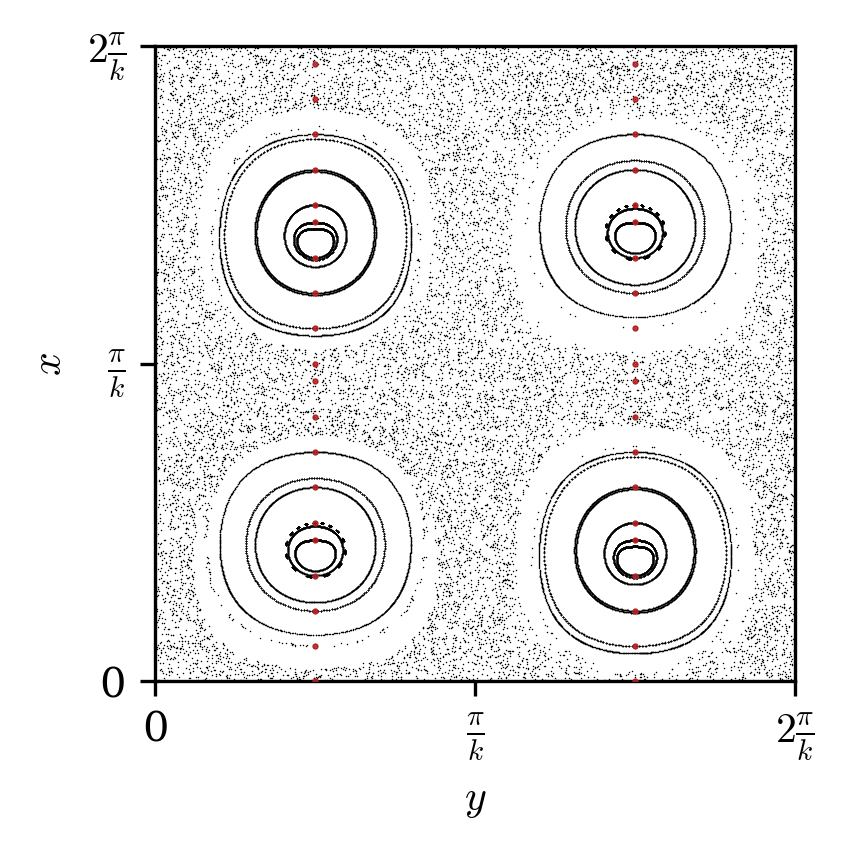
\includegraphics[width=\textwidth]{graf_2ondas/map2_data-map_U_p0.0000.png}
        \caption{$U = 0.0$}
    \end{subfigure}
    \begin{subfigure}[b]{0.3\textwidth}
        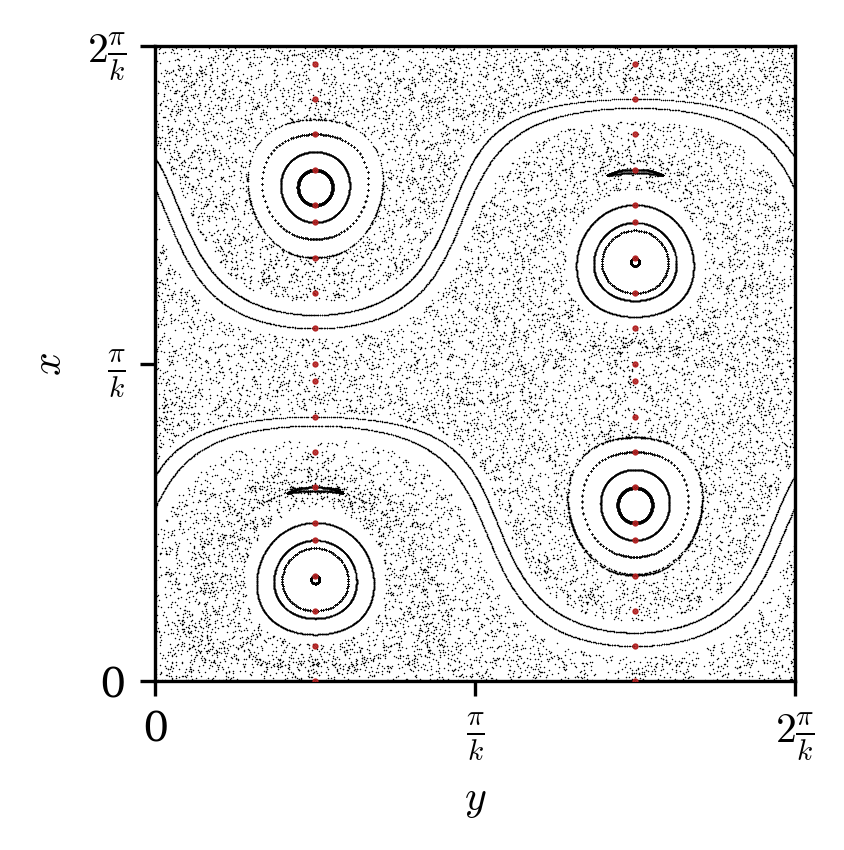
\includegraphics[width=\textwidth]{graf_2ondas/map2_data-map_U_p0.4000.png}
        \caption{$U = 0.4$}
    \end{subfigure}
    \begin{subfigure}[b]{0.3\textwidth}
        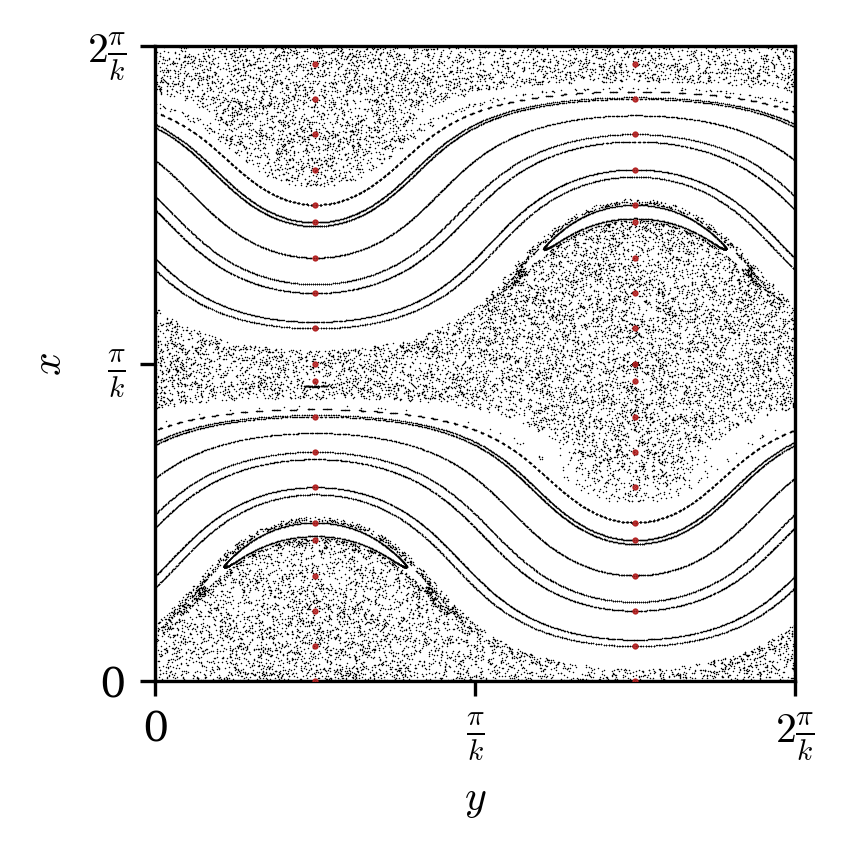
\includegraphics[width=\textwidth]{graf_2ondas/map2_data-map_U_p1.0000.png}
        \caption{$U = 1.0$}
    \end{subfigure}
\caption{Stroboscopic maps for  $A_2 = 0.3$. Initial conditions in red.}
\label{mapa2}
\end{figure}

\end{frame}

\begin{frame}{Individual trajectories}

We see the influence of $U$ by taking the same initial condition.

\begin{figure}[h]
\centering
\begin{subfigure}[b]{0.3\textwidth}
    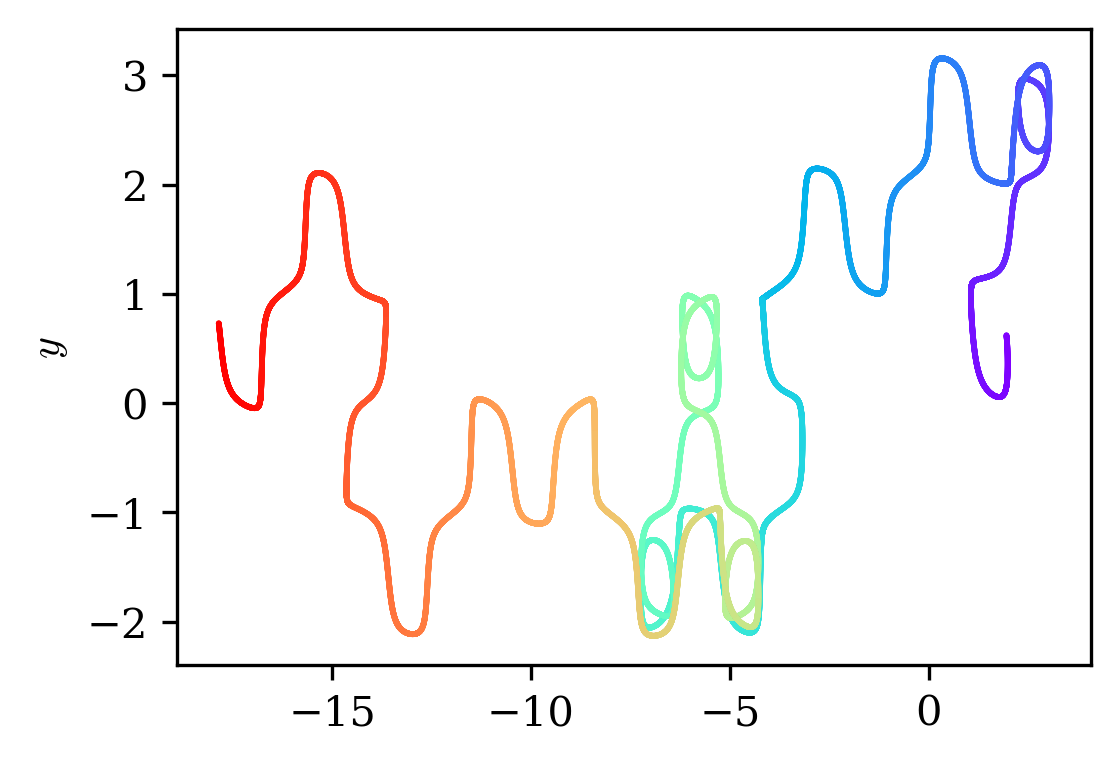
\includegraphics[width=\textwidth]{graf_2ondas/2w_0.0.png}
    \caption{$U = 0.0$}
\end{subfigure}
\begin{subfigure}[b]{0.3\textwidth}
    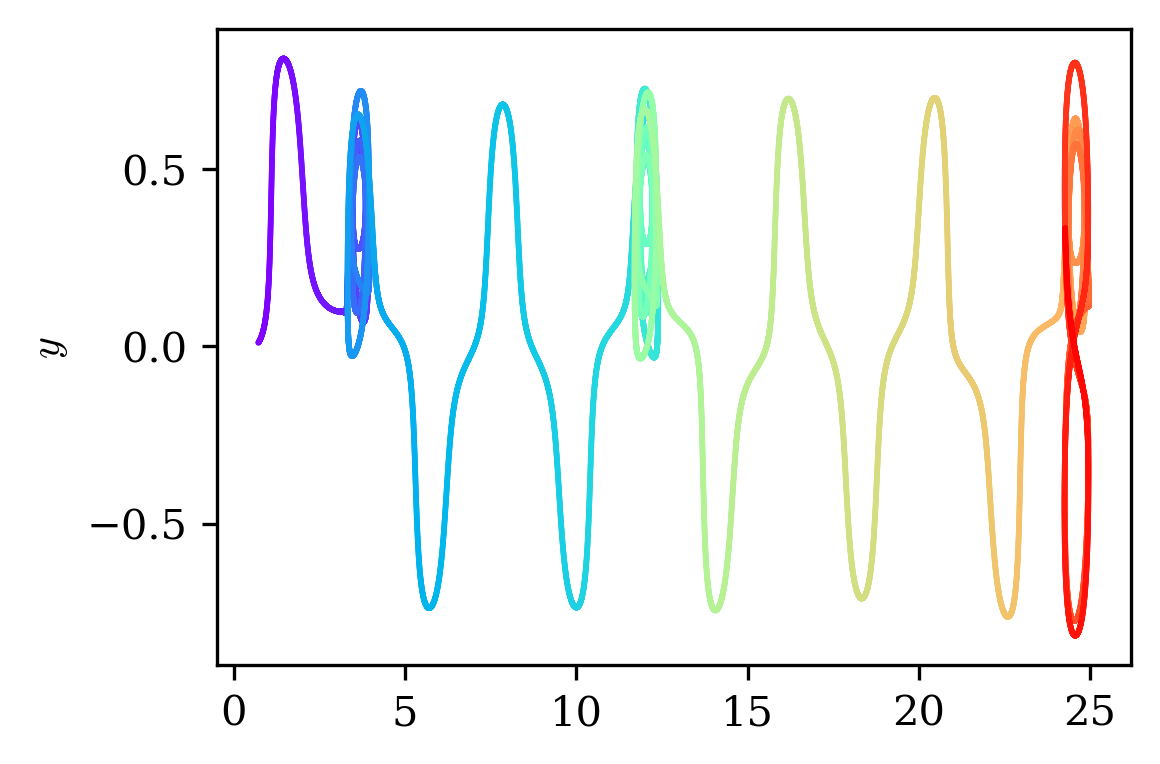
\includegraphics[width=\textwidth]{graf_2ondas/2w_0.4.png}
    \caption{$U = 0.4$}
\end{subfigure}
\begin{subfigure}[b]{0.3\textwidth}
    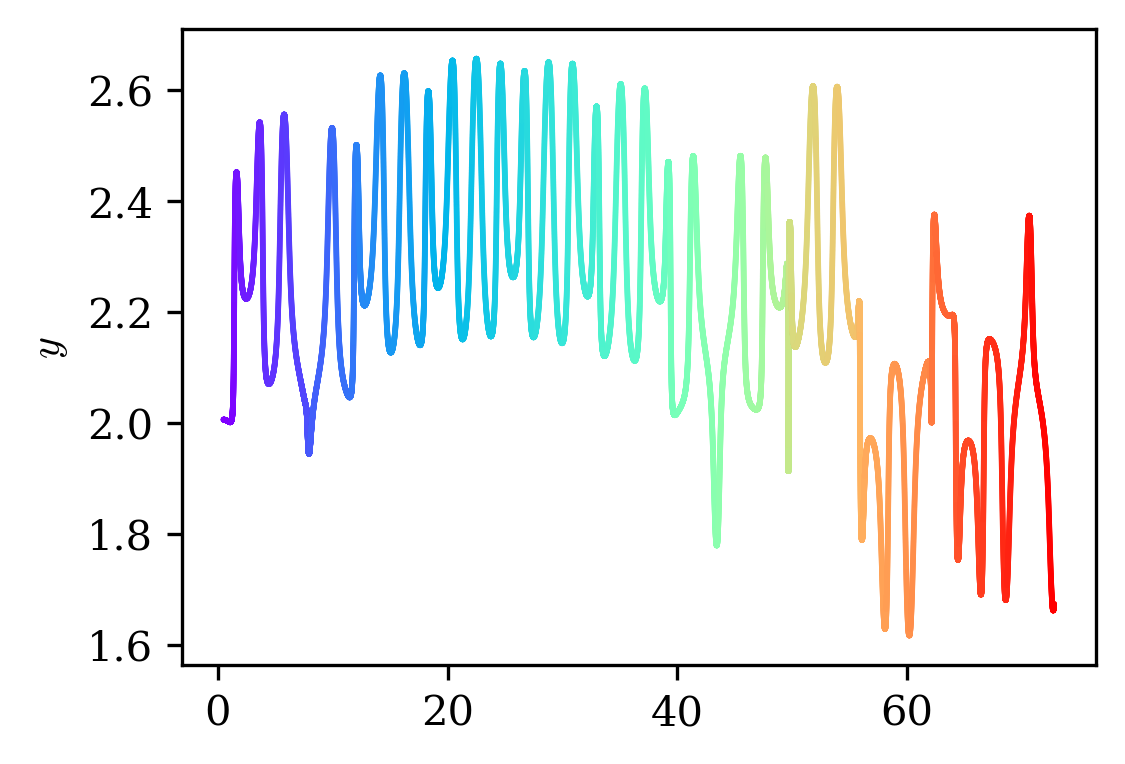
\includegraphics[width=\textwidth]{graf_2ondas/2w_1.0.png}
    \caption{$U = 1.0$}
\end{subfigure}


\caption{Trajectories for the same initial condition. Color represents time}
\label{traj2w}
\end{figure}

\end{frame}


\begin{frame}{Mean square displacement}

\begin{figure}[h]
\centering
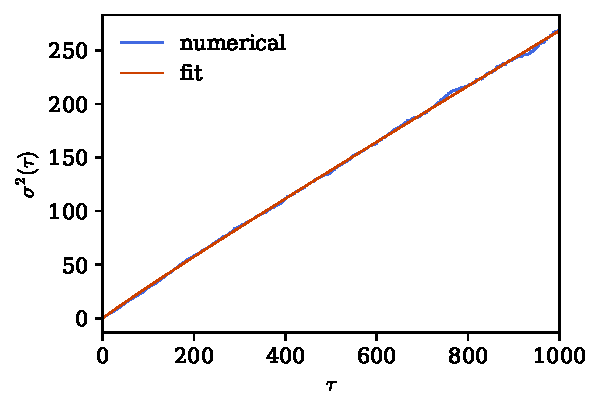
\includegraphics[scale = 0.75]{graf_2ondas/msd1.pdf}
\caption{Mean square displacement, for $U = 0.0$, $A_2 = 0.3$, $\theta_x = \pi/4$,  $\gamma = 0.968$}
\label{sigmaquadrado}
\end{figure}

\end{frame}



\begin{frame}{Diffusion in relation to $U$}


\begin{figure}[h]
\centering
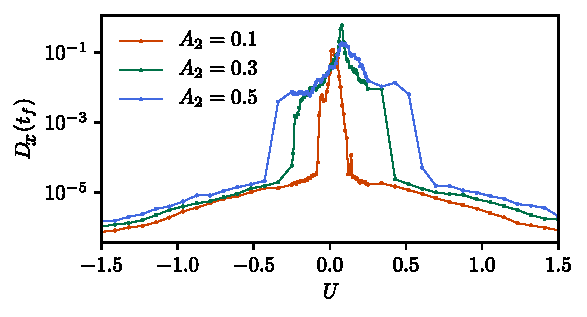
\includegraphics[scale = 0.9]{graf_2ondas/U_Dx.pdf}
\caption{$D_x$ for different values of $U$ and $A_2$}
\label{U_2wave}
\end{figure}

\end{frame}


\begin{frame}{Presence of anomalous transport}

\begin{figure}
    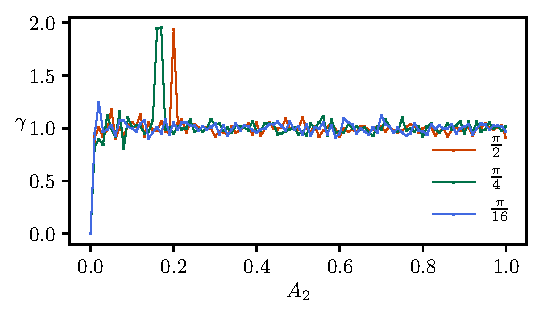
\includegraphics{graf_2ondas/gamma.pdf}
    \caption{ $\gamma$ in relation to $A_2$; for some values superdiffusion is present}
\end{figure}

\end{frame}

\begin{frame}{What is causing it?}

\begin{figure}
    \begin{subfigure}[b]{0.45\textwidth}
        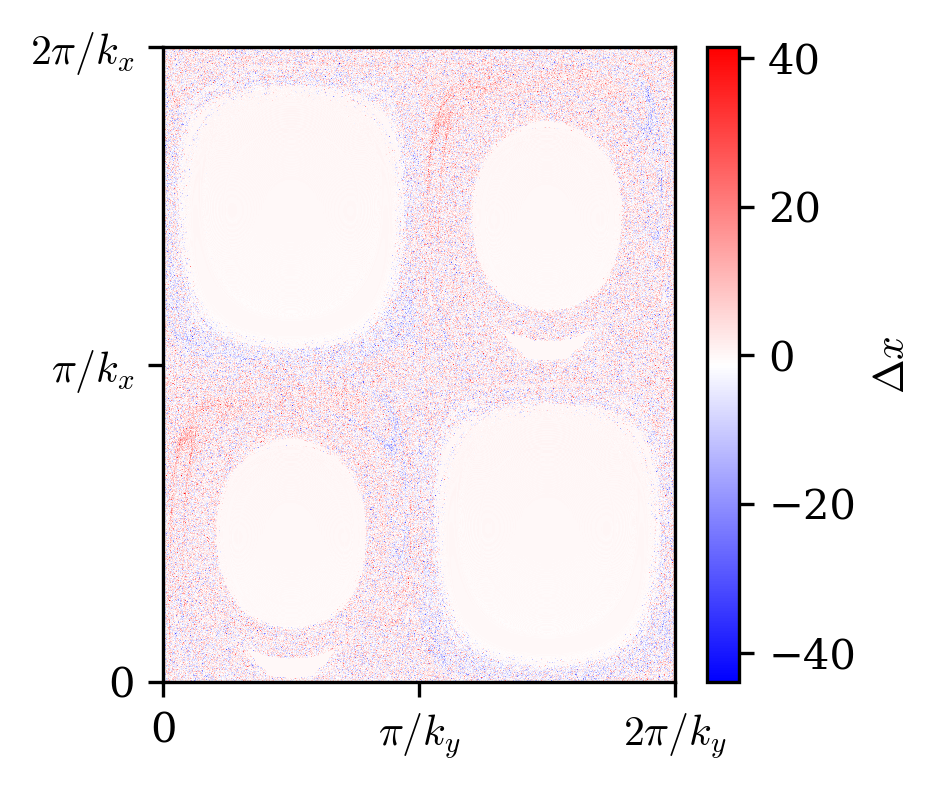
\includegraphics[width=\textwidth]{graf_2ondas/anom1.png}
        \caption{$A_2 = 0.20$}
    \end{subfigure}
    \begin{subfigure}[b]{0.45\textwidth}
        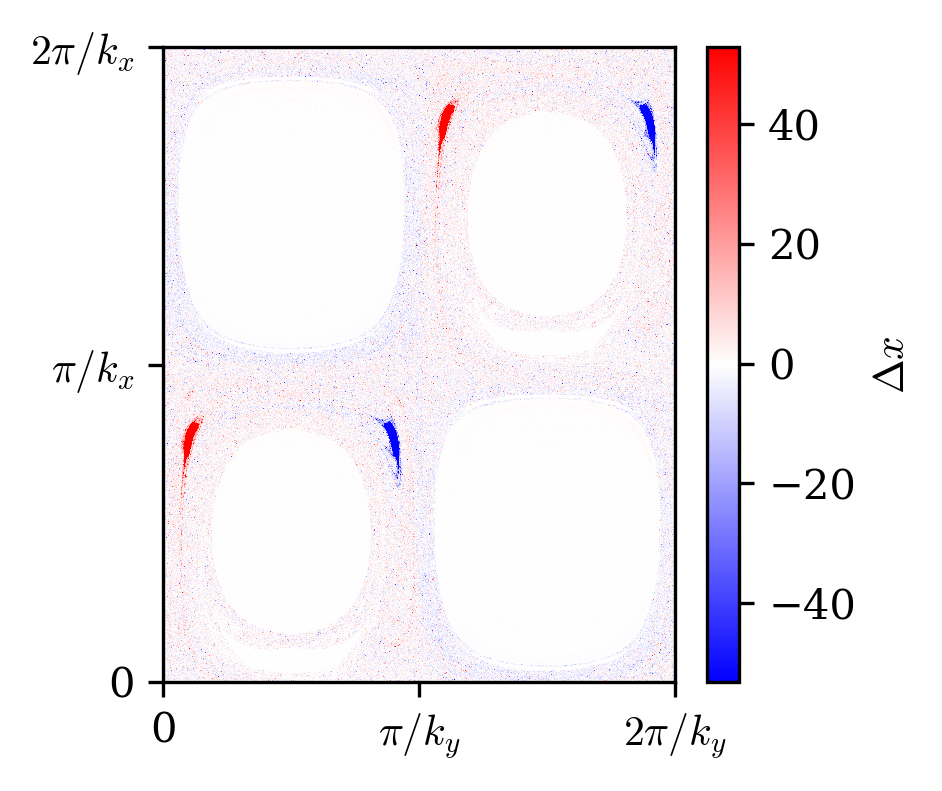
\includegraphics[width=\textwidth]{graf_2ondas/anom2.png}
        \caption{$A_2 = 0.16$}
    \end{subfigure}


    \caption{displacement on the phase space after 50 iterations, in color. $\theta_x = \frac{\pi}{4}$}
\end{figure}

\end{frame}

\begin{frame}{What is causing it?}

    \begin{figure}
        \begin{subfigure}[b]{0.45\textwidth}
            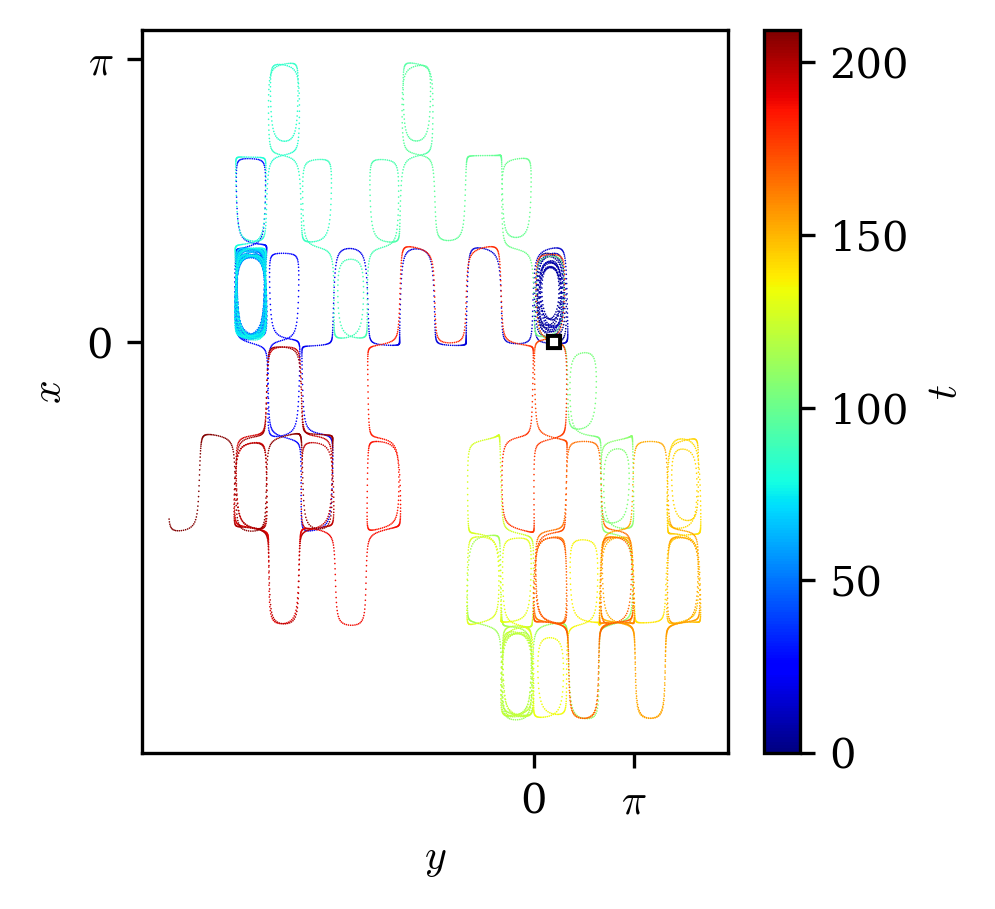
\includegraphics[width=\textwidth]{graf_2ondas/anom1_traj.png}
            \caption{$A_2 = 0.20$}
        \end{subfigure}
        \begin{subfigure}[b]{0.45\textwidth}
            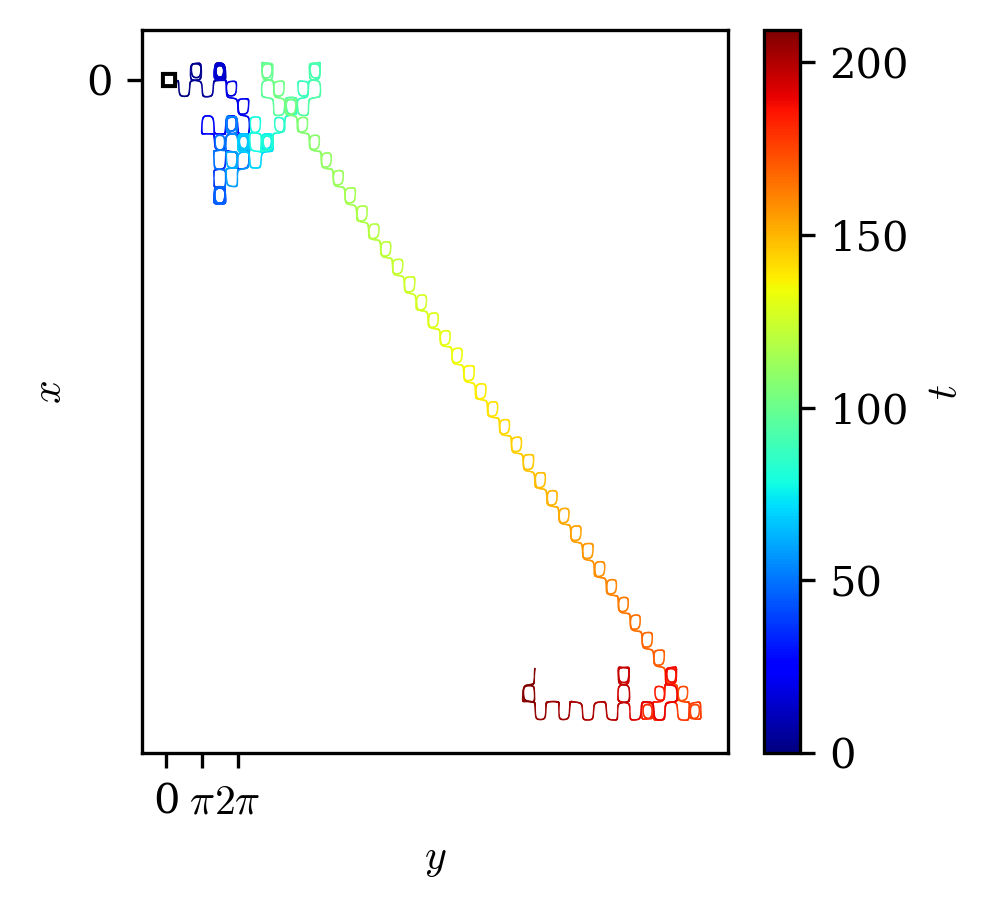
\includegraphics[width=\textwidth]{graf_2ondas/anom2_traj.png}
            \caption{$A_2 = 0.16$}
        \end{subfigure}

        \caption{Individual trajectories. $\theta_x = \frac{\pi}{4}$}
    \end{figure}
    
\end{frame}







\begin{frame}{Segment and test - Why and how to do it?}
 
    \begin{itemize}
        \item Diffusion is expensive
        \item Ballistic modes are sufficient condition for anomalous transport
        \item Adaptive 
    \end{itemize}

\begin{table}
    \begin{tabular}{c|c|c|c}
            &   Dsplacement & $\gamma$ evaluation & Segment and test\\
        \hline
        Parameters & $N_x \times N_y \times N_{it}$ & $N \times N_{it}$ & $N \times N_{it}$\\
        \hline
        Order & $10^{3} \times 10^{3} \times 10^{2}$  & $10^3 \times 10^4$ & $10^2 \times 10^4$\\
        \hline
        Order & $10^{8}$ & $10^{7}$ & $10^6$\\ 
    \end{tabular}
    \caption{Approximated iterations of some methods to identify anomalous transport}
\end{table}
    
\end{frame}

\begin{frame}{General idea}
    
    \begin{enumerate}
        \item Pick some initial conditions $\approx 100$
        \item Create the stroboscopic map
        \item Separate regions with morphology
        \item Test the regime in each region
    \end{enumerate}
\end{frame}

\begin{frame}{Standard map as a benchmark}

    \begin{equation}
        p_{n+1} = p_n + K\sin(\theta_n) \hspace{0.25cm},\hspace{0.25cm} \theta_{n+1} = \theta_n + p_{n+1} \hspace{0.25cm} \textnormal{mod}(2\pi)
      \end{equation}
    
        
      \begin{figure}
        \begin{subfigure}[b]{0.3\textwidth}
            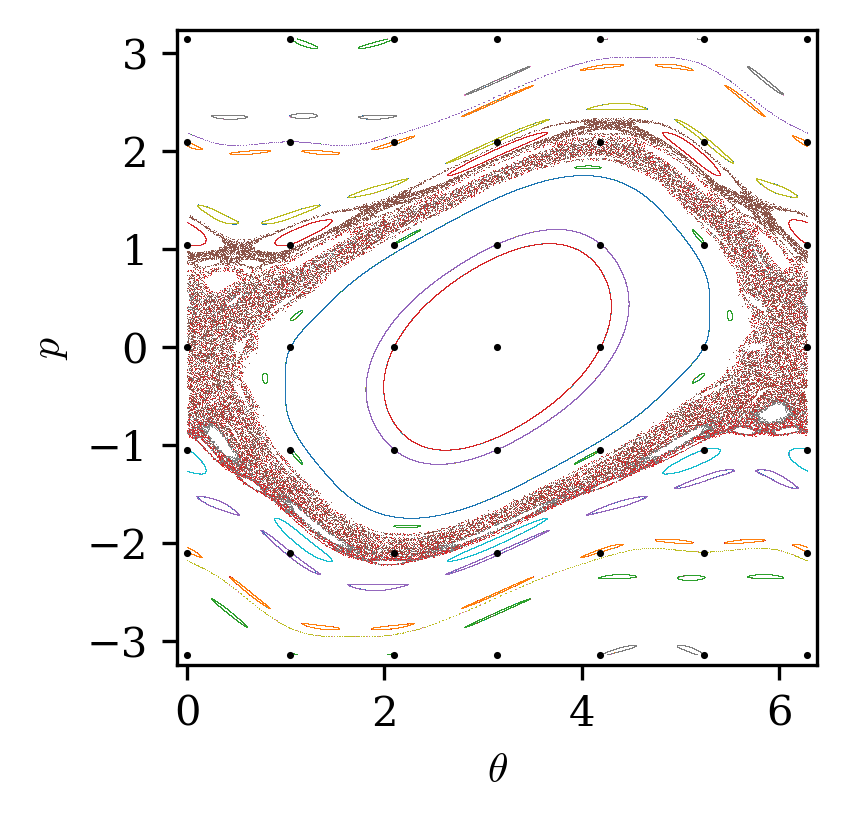
\includegraphics[width=\textwidth]{std/map_1_0.9000.png}
            \caption{$K = 0.9$}
        \end{subfigure}
        \begin{subfigure}[b]{0.3\textwidth}
            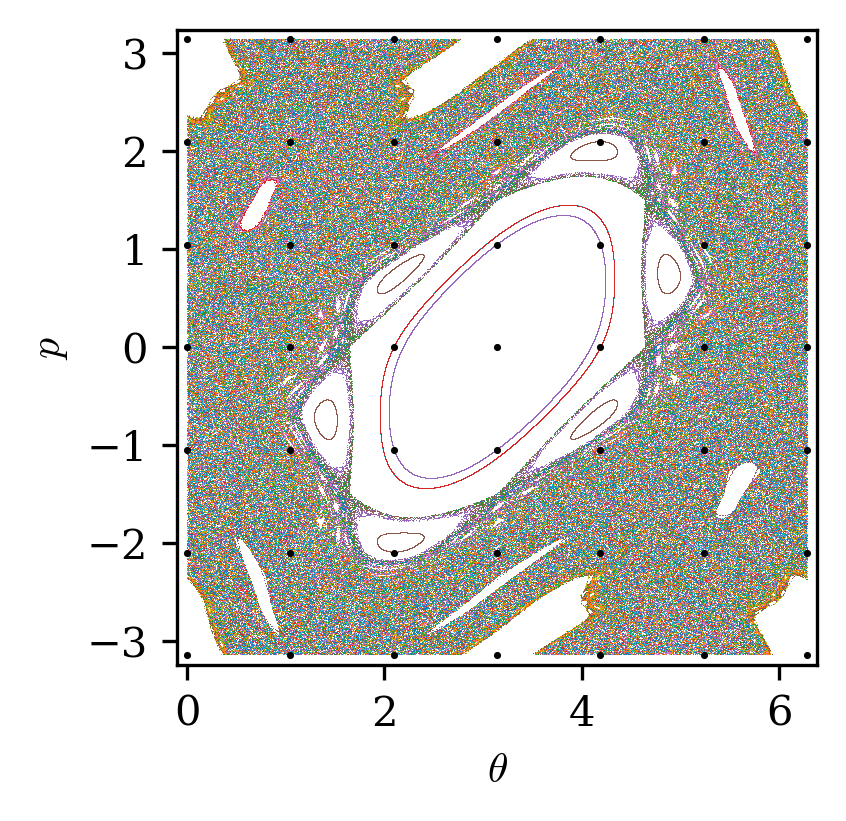
\includegraphics[width=\textwidth]{std/map_1_1.5000.png}
            \caption{$K = 1.5$}
        \end{subfigure}
        \begin{subfigure}[b]{0.3\textwidth}
            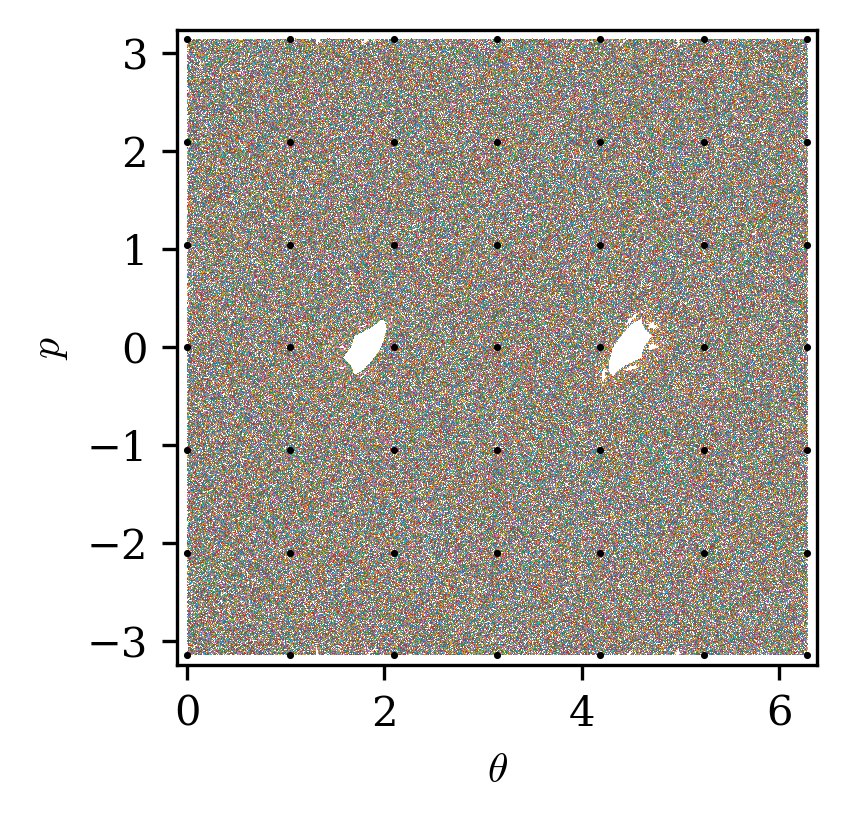
\includegraphics[width=\textwidth]{std/map_1_6.5000.png}
            \caption{$K = 6.5$}
        \end{subfigure}
        \caption{Phase space for some values of $K$.}
        \label{pspace}
    \end{figure}
\end{frame}


\begin{frame}{ST - Standard map - Segmentation}
    \begin{figure}
        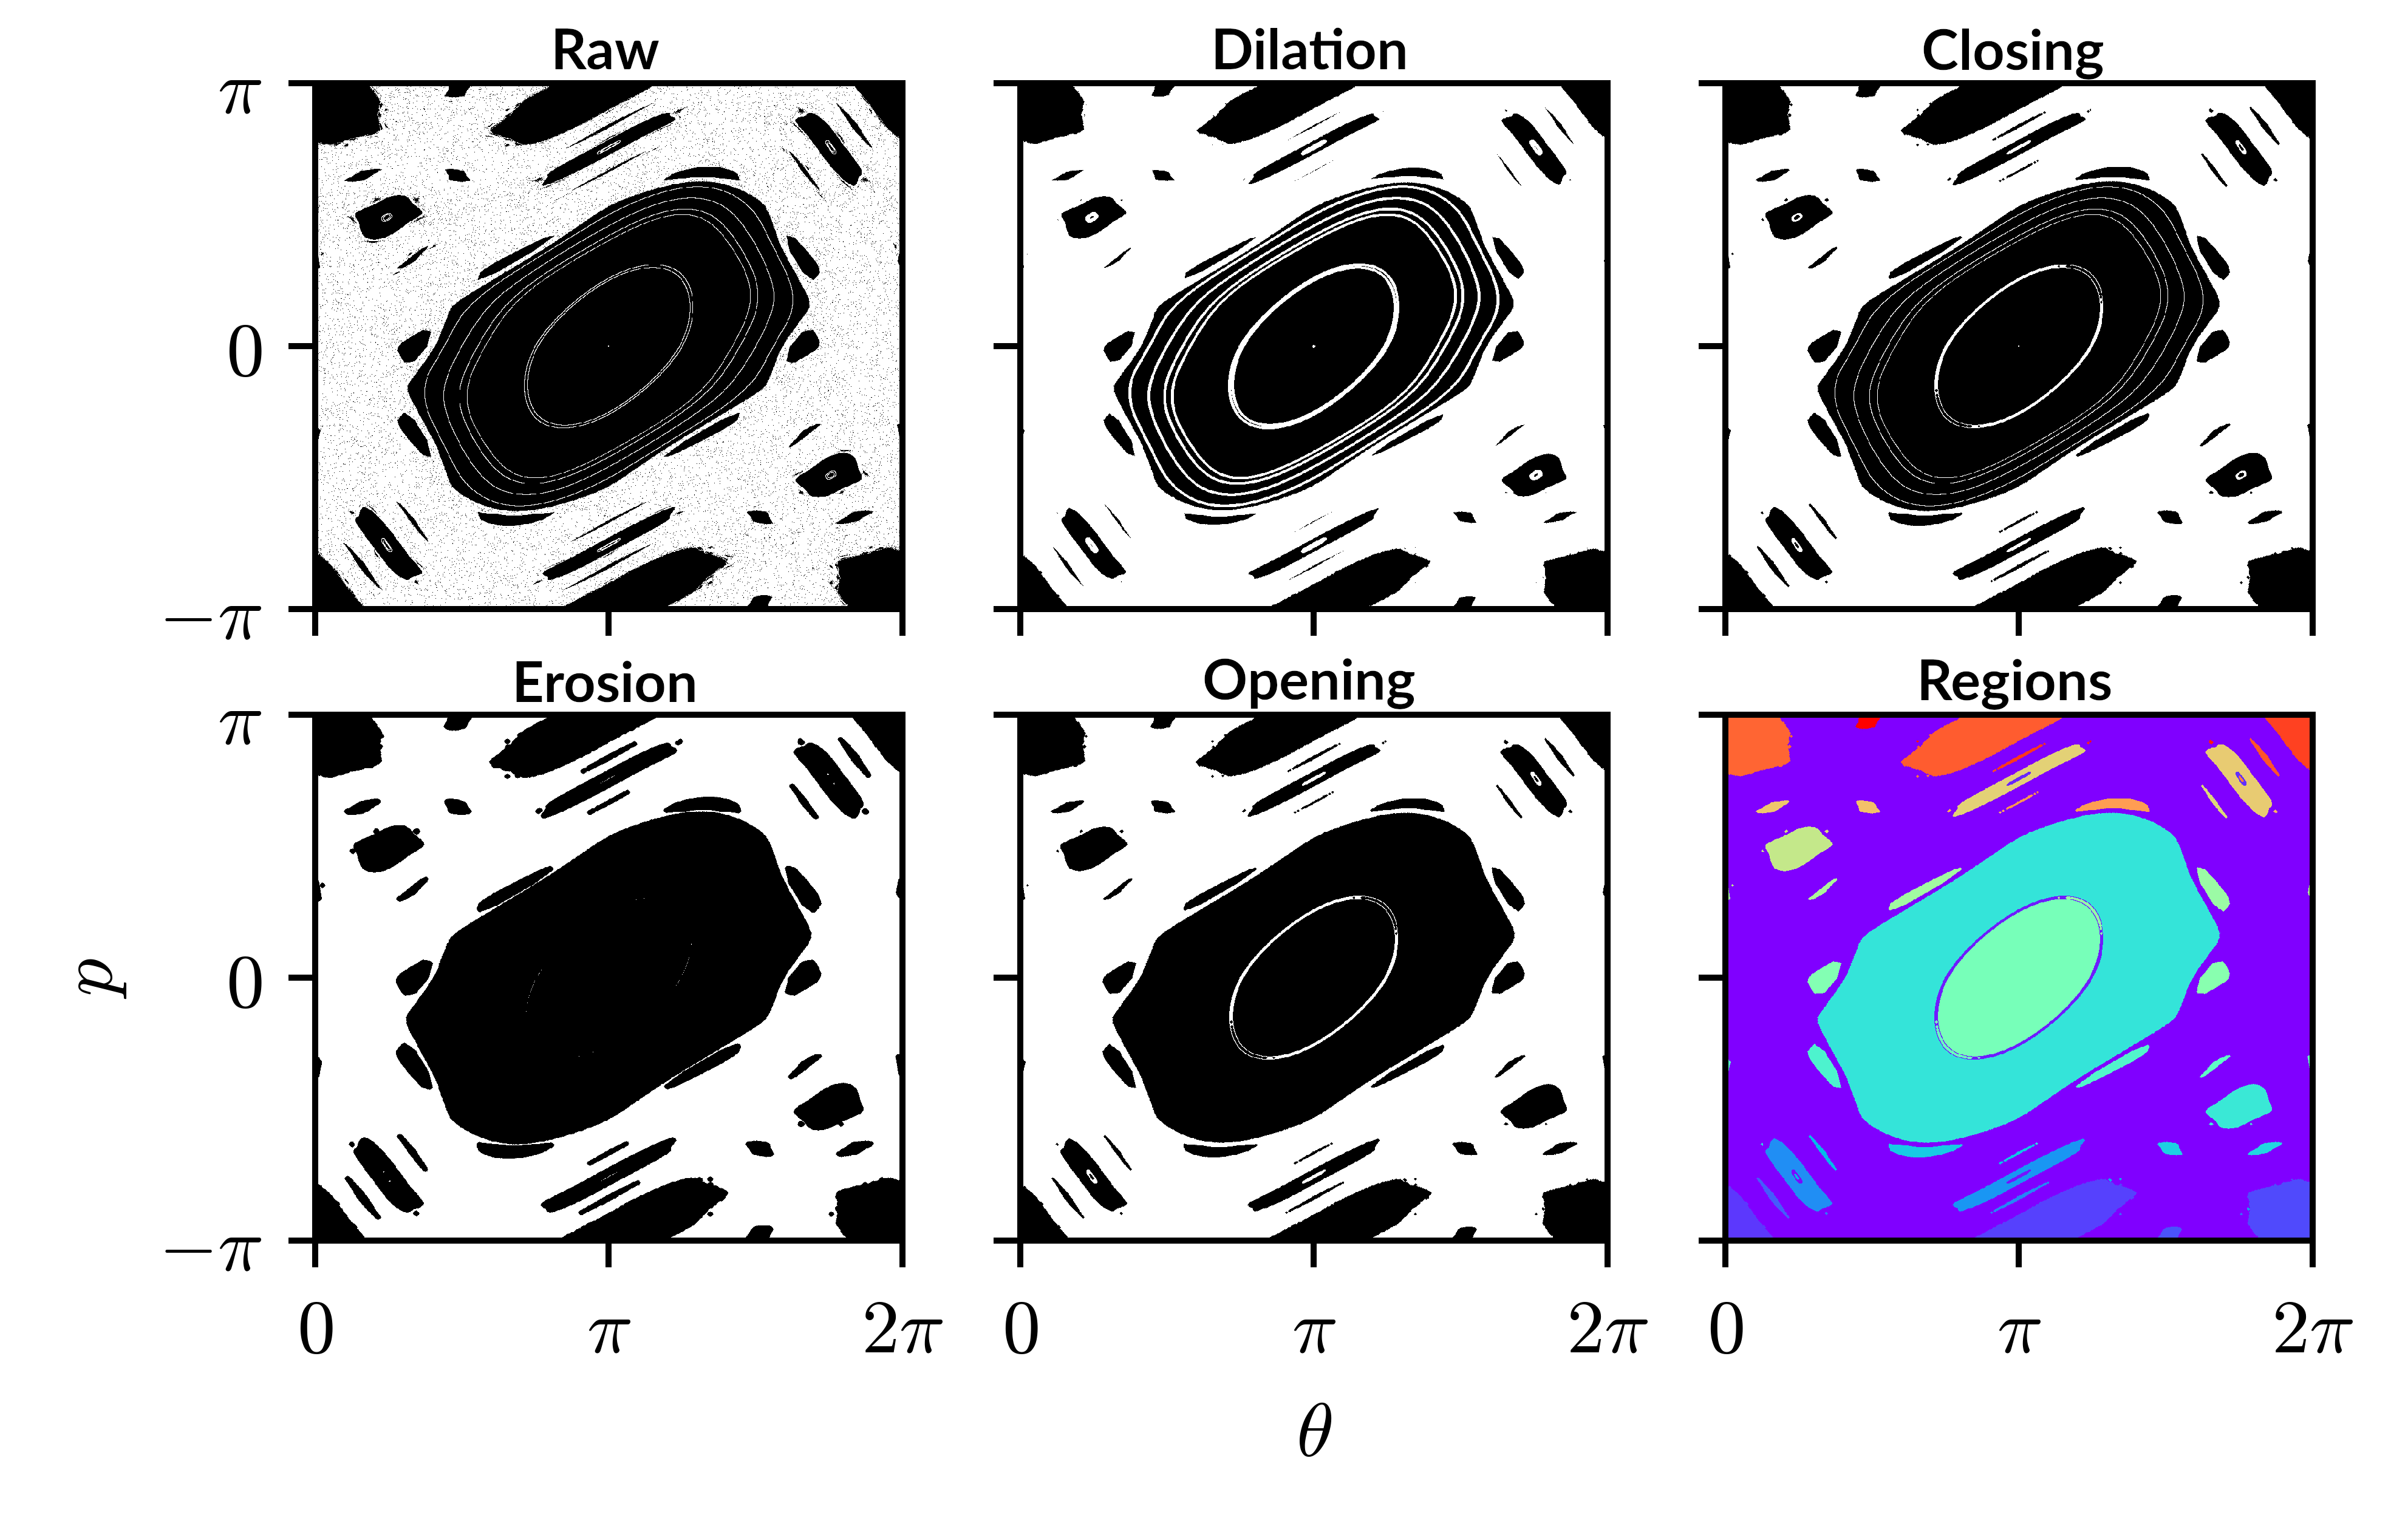
\includegraphics[width = \textwidth]{std/mm_6.png}
        \caption{Morphological steps for segmentation}
    \end{figure}
\end{frame}

\begin{frame}{ST - Standard map - Categorization}
    \begin{figure}
        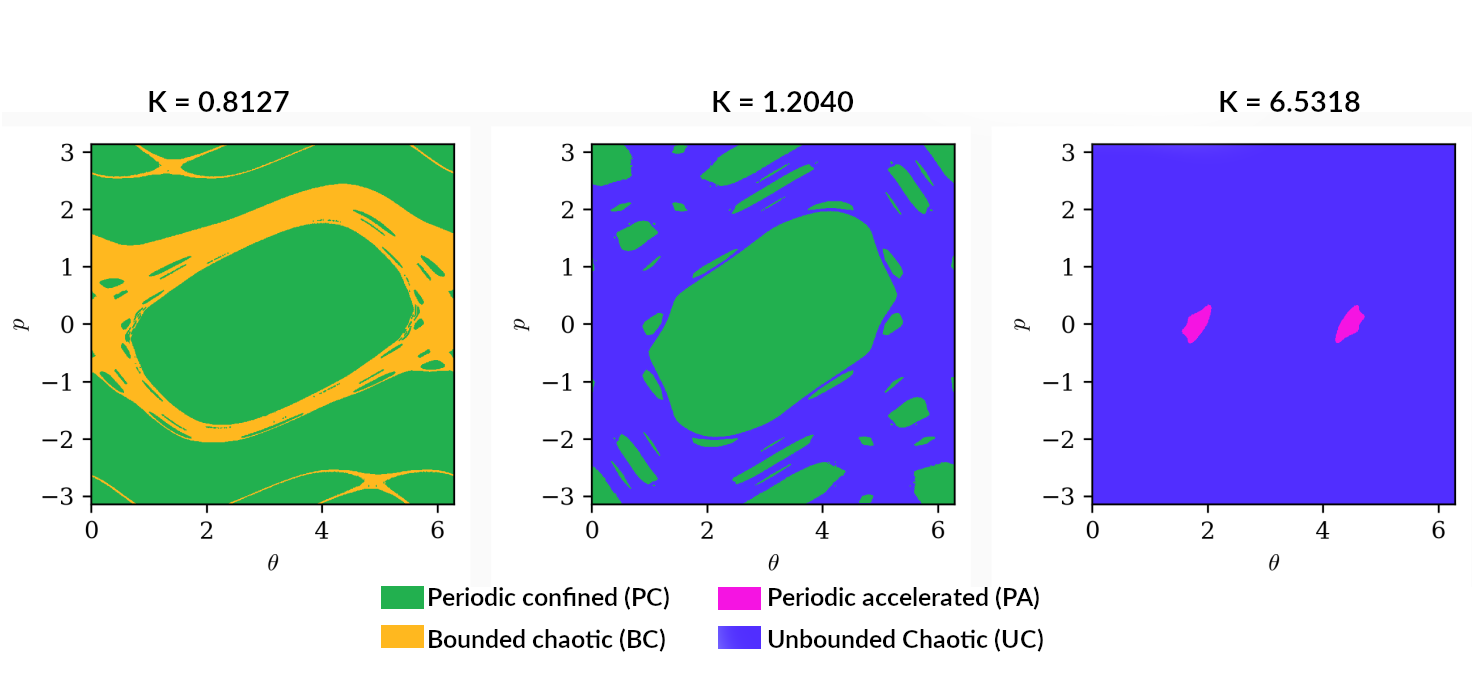
\includegraphics[width = \textwidth]{std/types.png}
        \caption{Categorized regions}
    \end{figure}
\end{frame}


\begin{frame}{ST - Standard map - Anomalous transport}
    \begin{figure}
        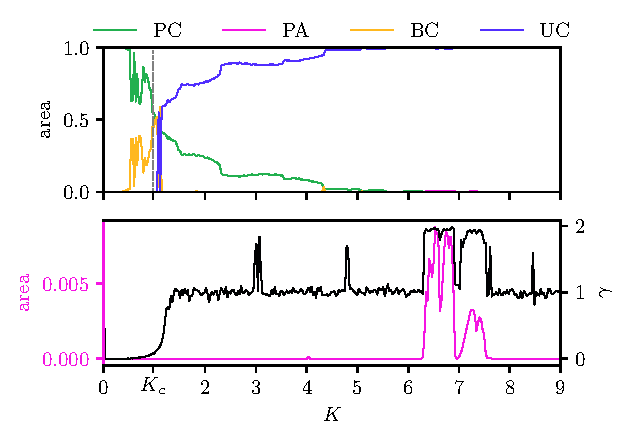
\includegraphics[width = 0.75\textwidth]{std/areas.pdf}
        \caption{Existence of anomalous transport when accelerator modes are present}
    \end{figure}
\end{frame}

\begin{frame}{ST - Two wave system}
    \begin{figure}
        \begin{subfigure}[b]{0.45\textwidth}
            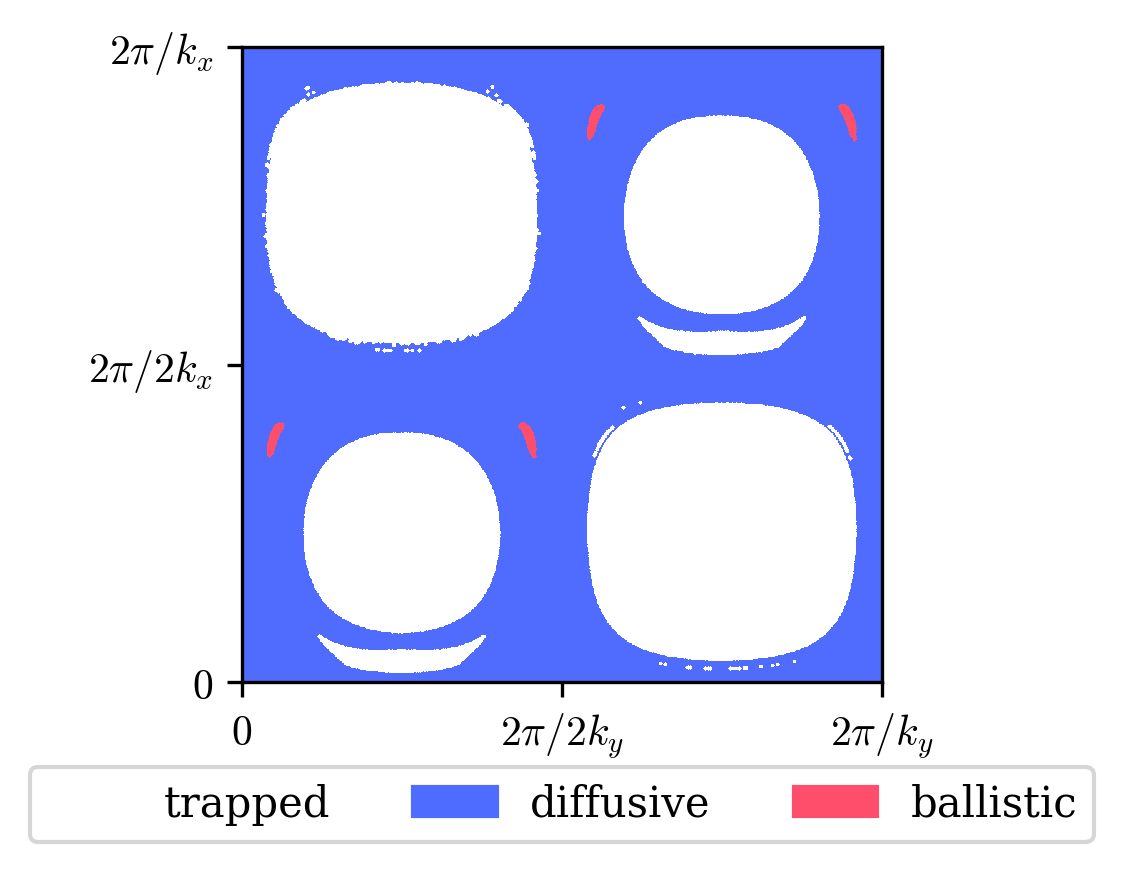
\includegraphics[width=\textwidth]{graf_2ondas/000.1600_000.7854.png}
            \caption{$A_2 = 0.16$}
        \end{subfigure}
        \begin{subfigure}[b]{0.45\textwidth}
            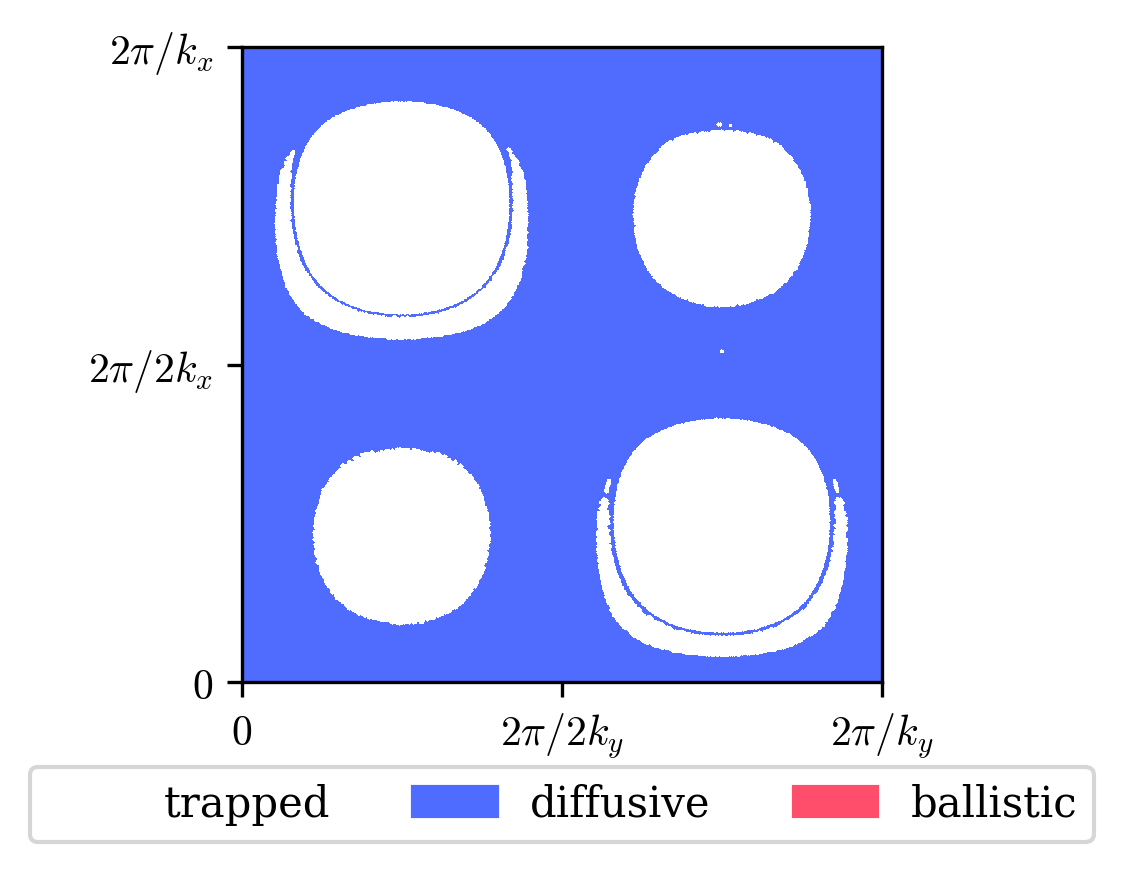
\includegraphics[width=\textwidth]{graf_2ondas/000.2100_000.7854.png}
            \caption{$A_2 = 0.2$}
        \end{subfigure}
        \caption{Categorization on the two wave system. $\theta_x = \frac{\pi}{4}$.}
    \end{figure}
\end{frame}

\begin{frame}{ST - Two wave system}
    \begin{figure}
        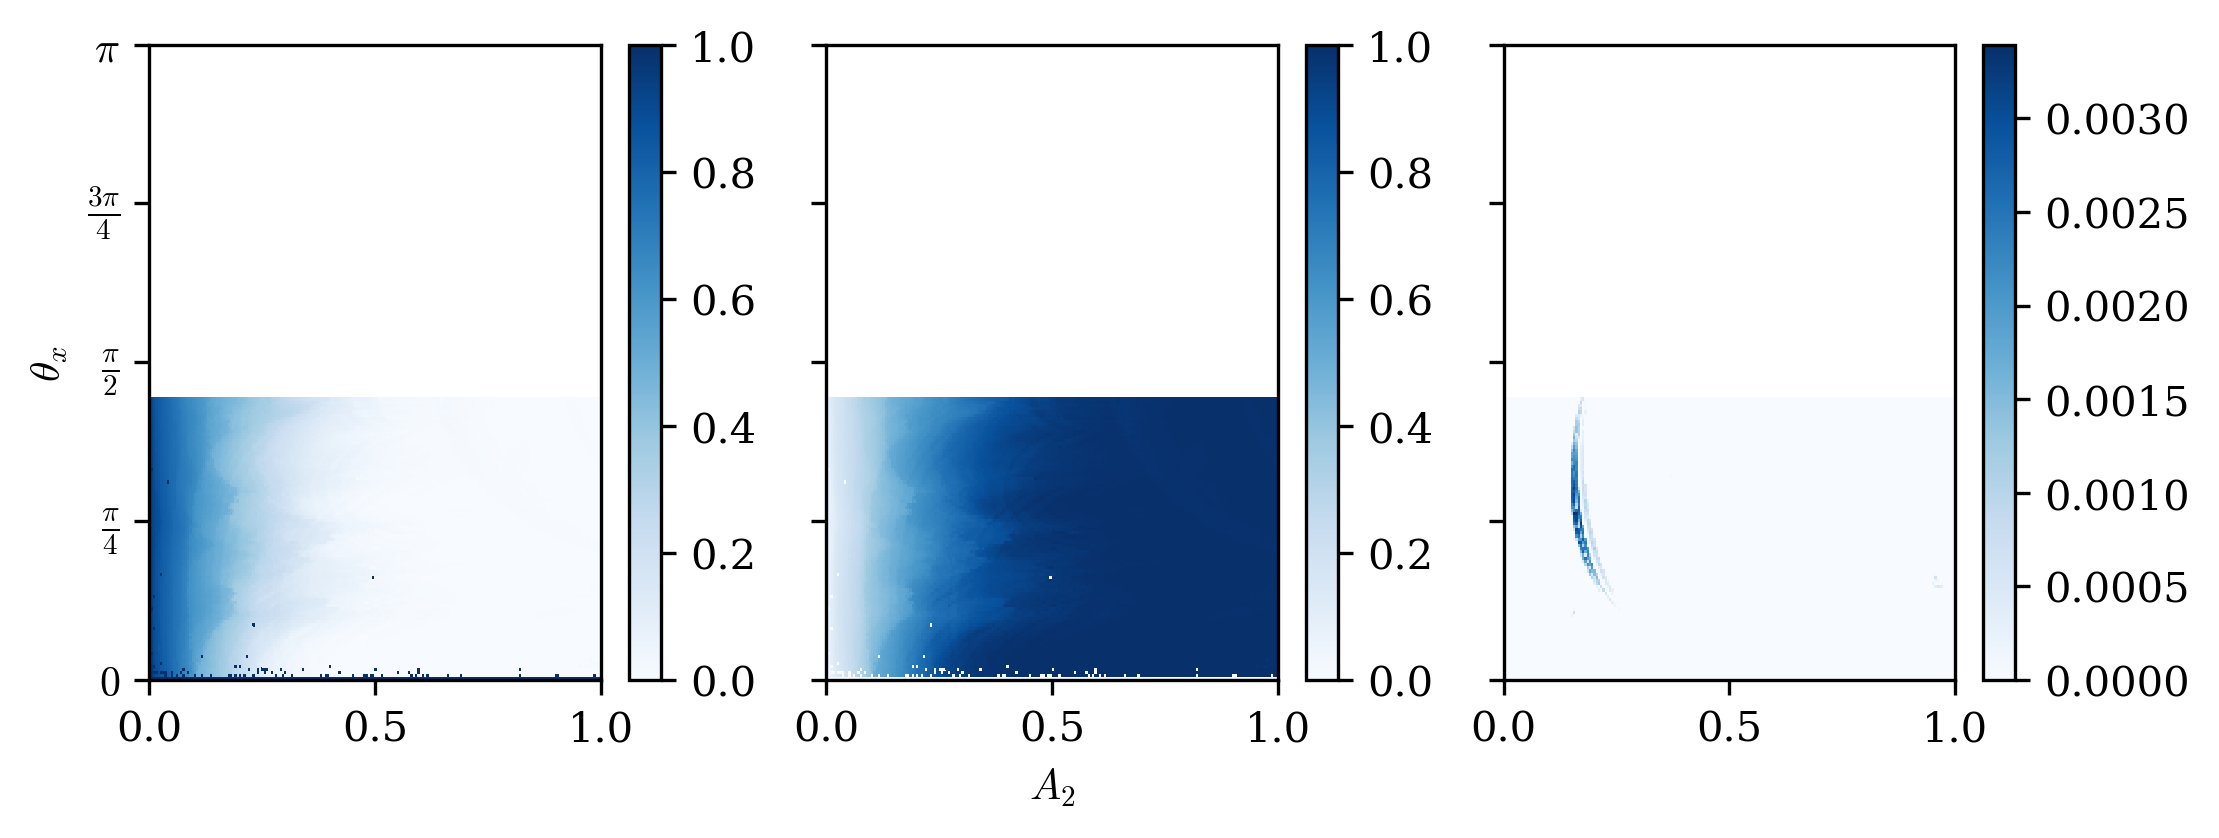
\includegraphics[width = \textwidth]{graf_2ondas/paramspace.png}
        \caption{Categorized regions; Estimated total wall clock simulation time: 20 Days}
    \end{figure}
\end{frame}







\section{Conclusions}

\begin{frame}{Conclusions}
\begin{itemize}
\item Investigation of the two wave system
\item Identification of ballistic modes
\item Development and application of ST approach  
\end{itemize}

\end{frame}



\section{Next steps}

\begin{frame}{Next Steps}
\begin{itemize}
\item Explore the control parameter $U$
\item Explore the influence of $k_x$ and $k_y$
\item System with more waves
\item Can anomalous transport happen for $U \neq 0$?

\end{itemize}
\end{frame}


\begin{frame}


\begin{center}
    {\huge  Thanks :)}

\end{center}



\end{frame}


\end{document}
